% chapter 1
\chapter{RLC Parallel Circuit Analysis}

\sisetup{scientific-notation=true}

\lstset{
    basicstyle=\ttfamily\small,
    frame=single,
    breaklines=true
}

%%%%%%   First section
\section{RLC parallel circuit analytical analysis}

\begin{table}[H]
\centering
\begin{tabular}{cc}
\hline
Parameter & Value \\
\hline
Current source $I$ & \SI{1}{\ampere} (AC) \\
Inductance $L$ & \SI{30}{\nano\henry} \\
Resistance $R$ & \SI{100}{\kilo\ohm} \\
Capacitance $C$ & \SI{50}{\femto\farad} \\
\hline
\end{tabular}
\caption{Circuit parameters}
\label{tab:parameters1}
\end{table}

Given the parameters in Table \ref{tab:parameters1}, we calculated the resonance frequency and quality factor of the parallel RLC circuit using analytical formulas:

\begin{equation}
f_r = \frac{1}{2\pi \sqrt{LC}} \qquad Q = R\sqrt{\frac{C}{L}}
\end{equation}

Substituting the numerical values we obtain:

\begin{equation}
f_r = 4.109 \ \si{\hertz} \qquad Q = 128
\end{equation}

%%%%%%   Second section
\section{LTspice Simulation}
Figure \ref{fig:ltspice1} shows the schematic representation of the parallel RLC circuit as implemented in LTspice.

\begin{figure}[H]
\centering
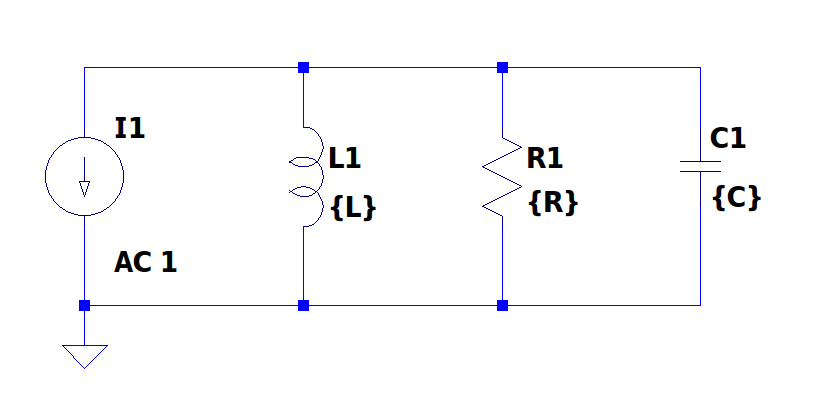
\includegraphics[width=0.6\linewidth, height=0.4\linewidth, keepaspectratio]{./exercise 1/RLCParallelCircuit.png}
\caption{Parallel RLC circuit implemented in LTspice}
\label{fig:ltspice1}
\end{figure}

The AC analysis was performed using the following simulation directive:

\begin{lstlisting}
.ac dec 1000 1 20G
\end{lstlisting}
\subsection{Resonance Frequency}
The resonance frequency is extracted in LTspice using the following directives:
\begin{lstlisting}
.meas AC max_v MAX mag(V(n001))
.meas AC f_res WHEN mag(V(n001))=max_v
\end{lstlisting}

\begin{figure}[h]
\centering
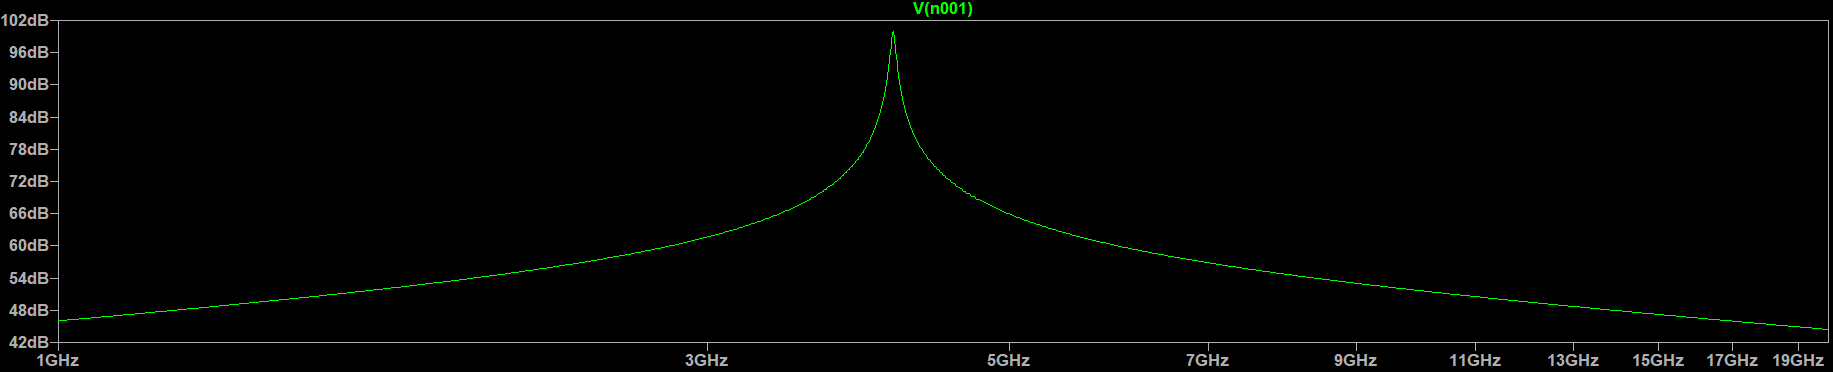
\includegraphics[width=0.8\linewidth]{./exercise 1/BodeResonanceFrequency.png}
\caption{Bode plot of the circuit showing the resonance frequency}
\label{fig:bode_resonance}
\end{figure}

The simulated resonance frequency was found to be  $f_r=$\SI{4.109}{\hertz} as shown in Figure \ref{fig:bode_resonance}, which is in excellent agreement with the analytical prediction. The amplitude value associated with the resonance frequency is found to be $V=\SI{99.98}{\kilo\volt}$.
The impedance \(Z\) of the circuit can be calculated as the ratio of the voltage \(V\) across the circuit to the current \(I=\SI{1}{\ampere}\) supplied by the source:
\begin{equation}
Z = \frac{V}{I}  = 99.98 \ \si{\kilo\ohm}
\end{equation}
Since the impedance at resonance is equal to the resistance \(R\) in a parallel RLC circuit, the simulated impedance value of \(Z \approx 99.98 \ \si{\kilo\ohm}\) is consistent with the expected value of \(R = \SI{100}{\kilo\ohm}\).


\subsection{Bandwidth}
The bandwidth of the resonance can be determined by finding the frequencies at which the voltage drops to approximately 70.7\%
of the maximum value, which corresponds to the -3 dB points of the resonance curve.

In order to find these frequencies, the following directives were used:

\begin{lstlisting}
.meas AC v_3db PARAM max_v*0.707
.meas AC f_low WHEN mag(V(n001))=v_3db RISE=1
.meas AC f_high WHEN mag(V(n001))=v_3db FALL=1
\end{lstlisting}

The results indicate that the lower and upper -3 dB frequencies are approximately $f_1 \approx \SI{4.093}{\giga\hertz}$ and $f_2 \approx \SI{4.125}{\giga\hertz}$, respectively.

The bandwidth is then calculated as

\begin{equation}
\Delta f = f_2 - f_1 \approx 31.8 \ \si{M\hertz}
\end{equation}
\subsection{Quality Factor}

Using the calculated values in LTSpice of the resonance frequency and the bandwidth, the quality factor can be estimated as

\begin{equation}
Q = \frac{f_R}{\Delta f} = 128.809
\end{equation}

This value is in very good agreement with the analytical prediction of \(Q = 128\), confirming the consistency between the theoretical analysis and the simulation results.

